
\chapter{Il Progetto}


\section{\label{sec:MatrixPro-e-Trackla2}MatrixPro e Trackla2}


\subsection{Creare Animazioni con MatrixPro}

MatrixPro \cite{MatrixPro} un software con licenza GPL2, ed quindi
gratuito e open source. Il tool  stato creato per permettere a studenti,
ma soprattutto ad insegnanti, di creare velocemente animazioni personalizzate
su strutture dati preesistenti nel programma. L'applicazione molto
utile come spiegano gli sviluppatori nell'articolo \cite{MatrixPro}
per rendere pi coinvolgenti le lezioni universitarie, con presentazioni
animate precedentemente create dal docente, o addirittura create al
volo durante la lezione, per riuscire a rispondere con la dimostrazione
visiva a domande e dubbi degli studenti.

Tra i punti di forza di questo applicativo troviamo la semplicit
con cui possono essere utilizzate le strutture dati esistenti, ma
soprattutto l'organizzazione di queste. Le strutture sono suddivise
in due grandi gruppi: 
\begin{description}
\item [{{FDT}}] (Fundamental Data Types) che equivalgono alle strutture
basilari, primitive alle quali non viene associata alcuna operazione
o informazione sematica riguardo al loro utilizzo. Tra queste troviamo
liste, alberi, grafi, array, chiavi. 
\item [{{CDT}}] (Conceptual Data Types) sono strutture che implementano
tipi di dato astratti che necessitano di maggiori restrizioni, e possono
essere modificate solo tramite operazioni che ne modificano la struttura
secondo regole predefinite. Tra queste troviamo Alberi Binari di Ricerca,
Heap, Stack, e molte altre. 
\end{description}
Esistono inoltre altre strutture utilizzabili nella realizzazione
di un'animazione, che vengono chiamate {}``strutture utili'' (utilities..
impossibile tradurlo), e permettono di creare al volo un input random
o consentono altre funzionalit allo stesso modo interessanti. Questa
classificazione in strutture primitive e avanzate aiuta l'utente a
comprendere meglio la gerachia esistente tra i diversi sistemi, e
a concentrarsi maggiormente sulla parte concettuale del problema analizzato
e non sui dettagli implementativi.

In accordo con il principio sul controllo del flusso espresso dalla
guida per sviluppatori, le animazioni create sono memorizzate all'interno
del sistema come una serie di passi, caratterizzati da un particolare
stato del sistema e di tutte le strutture coinvolte nella visualizzione.
All'utente  concessa la possibilit di esplorare i vari stati tramite
semplici comandi {[}Inizio-Indietro-Avanti-Fine{]}.

Una volta creata l'animazione desiderata,  possibile salvarla come
oggetto Java serializzabile, e si potr modificarla nuovamente in
un secondo momento. Inoltre MatrixPro permette di esportare il proprio
lavoro in 3 formati:
\begin{description}
\item [{\LaTeX{}}] immagine in formato .tex che  possibile includere facilmente
nei documenti Latex 
\item [{SVG}] che al momento a me non so perch ma non funziona.. (Scalable
Vector Graphics) l'esportazione in tale formato permette di salvare
un'animazione alla quale viene incluso anche un pannello di controllo
che permette di spostarsi avanti e indietro in modo simile a come
fa il software MatrixPro al suo interno.
\item [{PNG}] l'esportazione in formato PNG (Portable Network Graphics)
permette si creare una fotografia di un particolare momento dell'animazione
dell'algoritmo, che viene salvata in un file immagine PNG.
\end{description}

\subsection{Il sistema Trakla2}

A partire dalla versione {[}????{]} del software, si trova all'interno
del pacchetto che viene fornito da MatrixPro una funzionalit molto
interessante, che  stata chiamata Trakla2. Questa parte del sistema
consiste in un insieme di {}``esercizi'', creati a partire dal sistema
MatrixPro, all'interno dei quali lo studente deve simulare il comportamento
di un particolare algoritmo interagendo con le strutture grafiche.
Si accede a questi esercizi tramite il men Exercise nella barra dei
menu in alto.

\begin{figure}
\centering
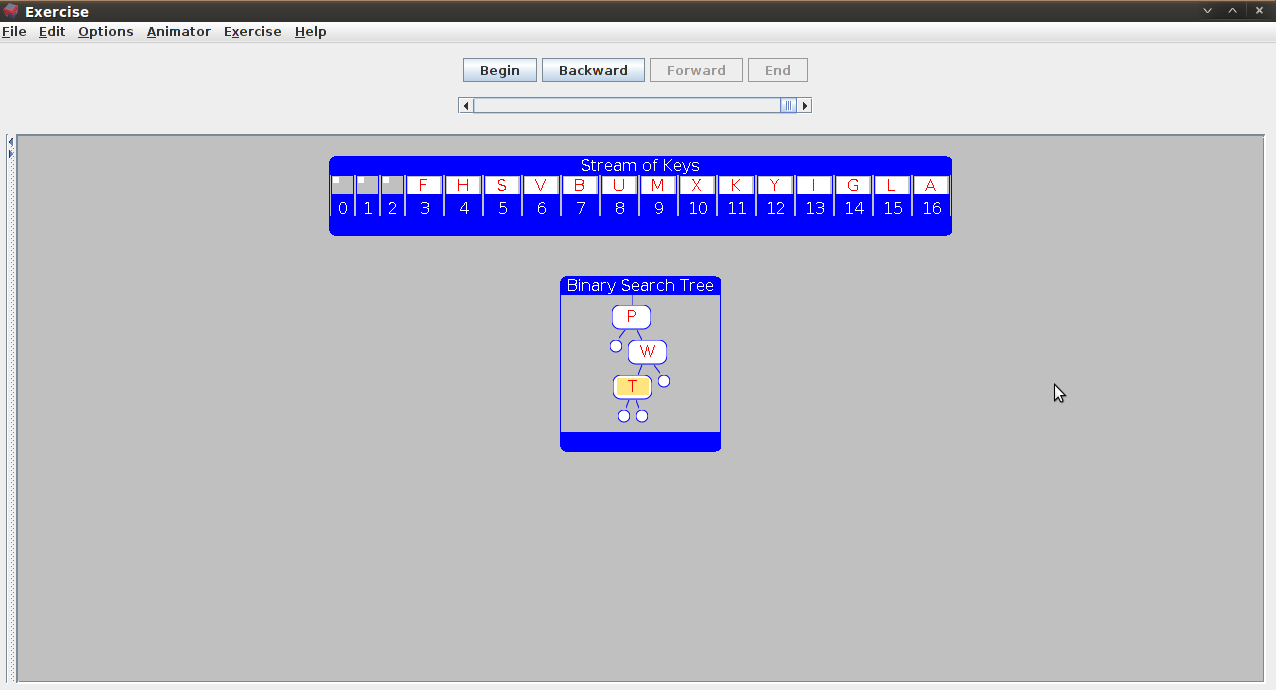
\includegraphics[scale=0.35]{images/trakla_screenshot.png}
\caption{Screenshot del sistema Trakla2}
\end{figure}

L'utente esegue i passi dell'algoritmo trascinando con il mouse {[}drag\&drop{]}
gli elementi delle strutture. I cambiamenti del sistema sono automaticamente
memorizzati ed  inoltre possibile tornare indietro e modificare le
azioni precedentemente eseguite.

Una volta terminata la simulazione, lo studente ha a sua disposizione
tre interessanti funzionalit, a cui si accede dal menu Exercise.
\begin{description}
\item [{Grade}] la funzione Voto permette allo studente di sapere se ha
ho meno eseguito una simulazione corretta. Nella maggior parte degli
esercizi la votazione viene espressa in numero di passi corretti nella
simulazione rispetto al numero dei passaggi totali. In altri esercizi
in cui non ha senso parlare di successione di stati, la valutazione
viene esplicitamente fornita con un messaggio testuale come per esempio
{}``Esercizio corretto'' o {}``Esercizio non corretto''.
\item [{Model\_Answer}] nella finestra Model Answer si visualizza l'animazione
corretta della simulazione dell'algoritmo preso in considerazione.
Attraverso questa modalit lo studente che non ha ancora compreso
il meccanismo di quesl particolare problema pu osservarne la simulazione
corretta. Questa caratteristica in conclusione  l'animazione che
gli altri software di AV forniscono agli utenti.
\item [{Compare}] (disponibile solo in alcuni esercizi) la funzione di
confronto pu essere vista come la fusione tra le altre due. Permette
infatti all'utente di confrontare passo-passo il risultato della propria
animazione con quello fornito dal sistema.
\end{description}
Anche negli esercizi del sistema Trakla2  possibile salvare ed esportare
l'animazione creata nei formati forniti da MatrixPro.


\section{Motivazioni della scelta di MatrixPro}


\subsection{Cosa si vuole realizzare}

Il progetto prevede la realizzazione di un software di visualizzazione
del comportamento degli algoritmi, destinato all'utilizz da partede
degli studenti del corso di Algoritmi e Strutture Dati, ed  realizzato
con l'intento di fornire un sussidio interattivo al libro di testo
del corso.

Il software dovr quindi coprire il pi possibili gli argomenti trattati
nel programma del corso, e dovr essere il pi interattivo possibile
per coinvolgere al meglio gli studenti.


\subsection{Scelta del tool pi adatto}

Per prima cosa  stata effettuata la ricerca di un applicativo preesistente
open source, dal quale partire e che sar in seguito modificato, per
realizzare il nuovo software di visualizzazione di algoritmi.

Dopo una prima analisi degli strumenti trovati, descritti nella sezione
\ref{sec:Strumenti-Disponibili}, sono stati subito scartati tutti
i programmi che fornivano solo una presentazione animata degli algoritmi,
ovvero software come Animal. Questa scelta  stata fatta per garantire
l'interattivit e il conseguente coinvolgimento degli studenti nell'utilizzo
dell'applicazione risultante.

La lista di software candidati si  quindi ristretta a 2 elementi:
JHAVE' e MatrixPro.

Il primo  un'applicativo facilmente scaricabile ed eseguibile direttamente
dal browser, che si connette a particolari server all'interno dei
quali sono contenute animazioni di numerosi algoritmi. In aggiunta
alla visualizzazione dell'algoritmo, JHAVE' fornisce allo studente
informazioni relative al problema, tra le quali per esempio lo pseudocodice
della soluzione, e interrompe l'animazione con domande inerenti alla
presentazione in corso dell'algoritmo.

MatrixPro, come spiegato in \ref{sec:MatrixPro-e-Trackla2}, concede
all'utente un livello maggiore di interattivit, pur fornendo anche
un'animazione {}``normale'' di molti algoritmi come gli altri applicativi
disponibili. Per quest'ultimo motivo la scelta finale  ricaduta sul
software MatrixPro.
